\documentclass[11pt]{article}
\usepackage[left=3cm,right=3cm,top=3cm,bottom=4cm]{geometry}
\usepackage{fixltx2e}
\usepackage{graphicx}
\usepackage{gensymb}
\usepackage{mathtools}
\usepackage[round]{natbib}
\usepackage{amssymb}
\usepackage{amsmath}
\usepackage{listings}
\usepackage[left]{lineno}
\usepackage{setspace}
\usepackage{placeins}
\graphicspath{{../Report/Graphics/}{../Results/}{../Results/Figures/}}
\doublespacing
\title{
\begin{flushright}

\includegraphics[scale = 0.4]{Imperial_Color2.pdf}
\end{flushright}
\textbf{How well does a mechanistic model based upon biochemical principles fit a dataset of thermal responses of individual fitness in phytoplankton?}
}
\author{Samuel Thompson}
\date{11/03/2015}
\begin{document}


\maketitle
\linenumbers
\textbf{WORD COUNT: 2980}
\section{Introduction}
The temperature dependence of metabolic rate is a key determinant of the maximum population growth rate in many systems, a feature that has long been known to biologists and ecologists. The traditional Malthusian exponential growth equation for a population \(N\), can be written as a function of time as
\begin{equation}
	N(t) = N(0)e^{rt}
\end{equation}
where \(r\) changes dependent upon the environmental variables. The maximum value, \(r_{max}\) has long been linked to both the body size of the animal and the temperature of the environment. With computer simulations allowing for unprecedented increases in the ability to use mathematical models to describe these systems, various mechanistic and phenomenological models have been developed. Models have been developed linking body size, temperature and population growth \citep{Savage2004a,Chen2010a} and even characterising genetic divergence based on temperature \citep{Allen2006a} . The two models of interest as examples of mechanistic and phenomenological models are, respectively, the Schoolfield model \citep{Schoolfield1981a} and the Gaussian-Gompertz model \citep{Martin2008a}.

The Schoolfield model is defined as 
\begin{equation}
	B(T) = B_0 \frac{\displaystyle {e^{\left(\displaystyle \frac {-E}{k}\left(\frac{-1}{283.15T}\right)\right)}}}{\displaystyle 1+\frac {E}{E_D-E}e^{\displaystyle \frac{E_D}{k}\left(\frac{1}{T_{pk}} - \frac{1}{T}\right)}}
\end{equation}
where \(k = 8.617 \times 10^{-5} eVK^{-1}\) is the Boltzmann constant, \(B(t)\) is the value of the trait at temperature \(t\), (growth for the datasets of interest), and \(B_0\) is the trait value at 283.15K, or 10 \celsius. \(E\) and \(E_D\) are the activation and deactivation energies, which control the rise and fall of the curve. \(T_{pk}\) is the temperature where the trait value is maximal. The temperature value \(T\) is defined in Kelvin.

The Schoolfield model is mechanistic, with each parameter has a biological representation based on the Arrhenius equation and Eyring's theoretical equation \citep{Schoolfield1981a}. On the other hand, the Gaussian-Gompertz model is phenomenological, with parameters \(B_{max}\), the maximum trait measurement, and \(\theta\), simply a quantity that improves the fit. Neither parameters have any biological significance, and temperature is here measured in celsius. The model is defined as
\begin{equation}
	B(T) = B_{max}e^{\displaystyle\left( -E(T-T_{pk})^2-e^{\displaystyle \left( E_D(T-T_{pk}-\theta \right)}\right)}
\end{equation}

In order to assess how well the mechanistic model can fit the dataset of thermal responses, it was compared against the Gaussian-Gompertz model and a cubic model an example of another phenomenological model. The cubic model was simply defined as the general cubic equation,
\begin{equation}
	B(T)=a + bT + cT^2 + dT^3
\end{equation}
with \(a\), \(b\), \(c\) and \(d\) not having any biological bearing. The cubic model can therefore be used to compare to the other models, as it has a similar number of parameters.

%%%%%%%%%%%%%%%%%%%%%%%%%%%%%%%%%%%%%%%%%%%%%%%%%%%%%%%%%%%%%%%%%%%%%%%%%%%%%%%%%%%%%%%%%%%%%%%

\section{Method}
To investigate the ability of the mechanistic model to fit thermal responses, a dataset was used from 855 experimental studies on phytoplankton from around the world, compiled by \cite{Chen2010a} and \cite{Thomas2012a}. For each experiment, growth traits were recorded for a number of individuals at different temperatures, which would then be fitted using Non-linear Least Squares (NLLS) analysis. This approximates the model to a linear model and refines the parameters over successive iterations to minimise the difference between the model trait values and actual trait values. Models are then selected by the Akaike Information Criterion \citep{Akaike1973}, and Bayesian Information Criterion \citep{Schwarz1978} to decide which produces the best fit for the dataset.

Before fitting, the data was first analysed to produce an estimate to aid model fitting, based off the maximum trait values, and using a linear model to estimate \(B_0\), \(B_{max}\), \(T_{pk}\), \(E\) and \(E_D\). The starting values for these parameters would be used to speed up model fitting and were based off the gradient, intercept and minimum value of the linear model, which disregarded points with temperature greater than the maximal trait value. The linear model produced to estimate these parameters uses a logarithmic function to linearise the points to a straight line, as shown in Figure \ref{fig:prep}.

\begin{figure}[h]
\begin{center}
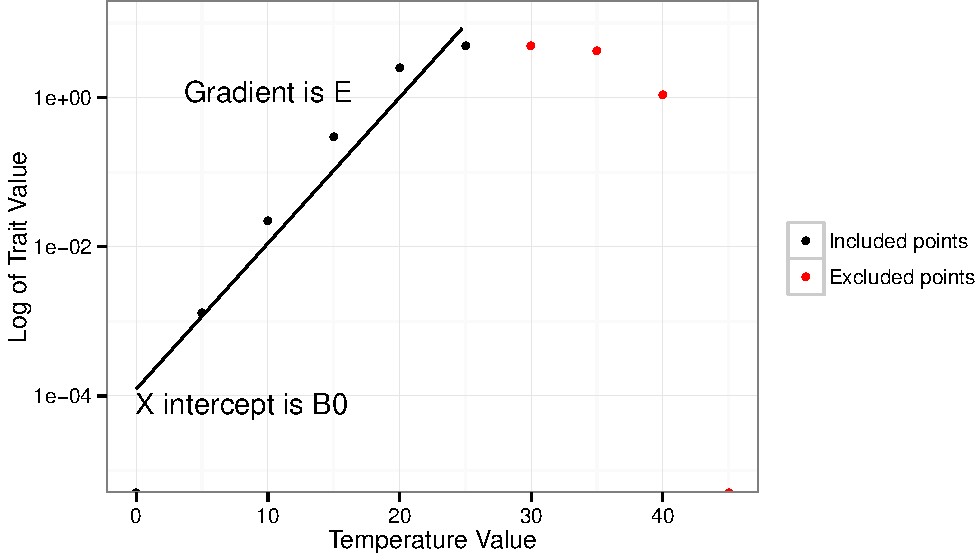
\includegraphics[scale = 1]{prep_example.pdf}
\caption{Example plot of initial linear model to produce parameter values. \(E_D\) is then estimated as \(\frac{1}{2}E\) and \(T_{pk}\) is estimated as the maximal trait value observed.}
\label{fig:prep}
\end{center}
\end{figure}

At this point, the datasets were constrained to remove those with too few data points for meaningful model generation. A minimum of 5 unique points was required to ensure that the model had fewer parameters than the number of data points, otherwise over-fitting would occur. Recordings without trait or temperature values were also removed, as for the purpose of model fitting they would be meaningless. After filtering out these datasets, a total of 651 datasets were available to find parameter estimates for and begin fitting to the three models.

For the Schoolfield model, the parameters \(B_0\), \(E\), \(E_D\) and \(T_{pk}\) were all allowed to vary. The \(E\) and \(E_D\) values constrained to positive values as they represent biological activation energies, which are assumed to be positive, and have \(E>E_D\).

The Gaussian-Gompertz model has parameters \(B_{max}\), \(E\), \(E_D\) and \(T_{pk}\), and all were allowed to vary over any number except for \(B_{max}\), which was constrained to the experimental maximum trait value due to its phenomenological interpretation. For the cubic model all parameters, \(a\),\(b\),\(c\) and \(d\) were allowed to vary, as none have any biological interpretation.

During the fitting process, \texttt{Python} \citep{python} was used with the \texttt{lmfit} function. For the cubic and Schoolfield models, non-linear least squares fitting was performed using the Levenberg-Marquardt algorithm \citep{Levenberg1944}. However, this didn't produce fantastic fits for the Gaussian-Gompertz models, so the Nelder-Mead algorithm \citep{Nelder1965} was instead utilised here, which is slower but worked well at producing fits without infinite standard errors in the parameters.

%%%%%%%%%%%%%%%%%%%%%%%%%%%%%%%%%%%%%%%%%%%%%%%%%%%%%%%%%%%%%%%%%%%%%%%%%%%%%%%%%%%%%%%

\section{Results}
Using the method outlined above, all 661 datasets produced models for the Gaussian-Gompertz and cubic models, while 651 were produced for the Schoolfield model. The Schoolfield models which failed to produce fits had strange data, such as decreasing trait values with temperature, and therefore can be ignored, especially as there were so few. As a measure of the decency of fits for each of the datasets, individual R-squared (\(R^2\)) values were calculated, and graphs plotted overlaying each of the models for every dataset. It appeared that for data with simple sigmoidal increases in trait value with temperature, likely as no experimental values existed for temperatures greater than the \(T_{pk}\), all three models fitted with low errors and a high level of fit. An example is shown in Figure \ref{fig:interest}A. 

\begin{figure}[h]
\begin{center}
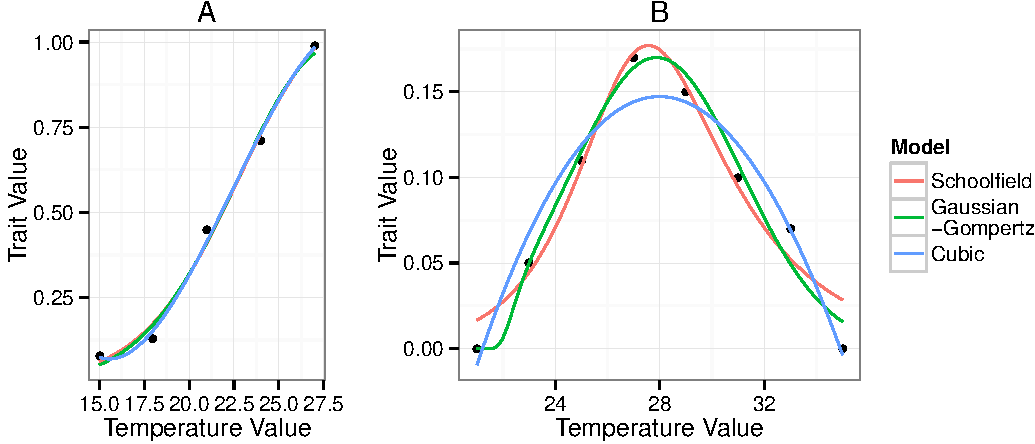
\includegraphics[scale = 1]{interest.pdf}
\caption{\textbf{A)} Example of the sigmoidal shape of some of the datasets which easily produced fits. Here the data was of \textit{Synechococcus} species \citep{Mackey2013}. \textbf{B)} Example of all models fitting well, with a defined peak as seen in some datasets. Here the data was of \textit{Prorocentrum mexicanum} species \citep{Morton1992}}
\label{fig:interest}
\end{center}
\end{figure}


Other models with well defined peaks also produced good fits for all three models, as shown in Figure \ref{fig:interest}B. In these cases, most often the Schoolfield model produced the best fit as measured by the AIC and BIC, likely due to the same number of variables that exist in the model, but increased fit. In these cases, it appears that a mechanistic model fits the dataset better than the two phenomenological models. Moreover, there were many cases where the cubic and Schoolfield model produced reasonable fits for the data, whilst the Gaussian-Gompertz model struggled with low numbers of data points and very low trait values. 

\FloatBarrier

The jumps seen in the model produced in Figure \ref{fig:jumps} would likely not be representative of real-world systems. The smoother curve produced by the Schoolfield model is more likely to be biologically accurate, as well as allowing for much more accurate extrapolation outside of the experimental data range.

\begin{figure}[h]
\begin{center}
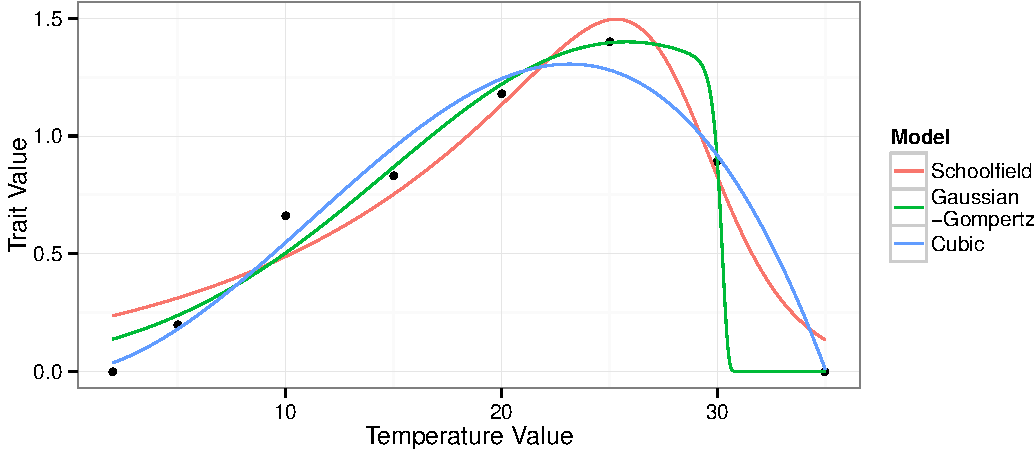
\includegraphics[scale = 1]{jumps.pdf}
\caption{Gaussian-Gompertz model producing poorer fits for trait values equal to 0. The data is of \textit{Pandorina morum} from \cite{Moss1973}.}
\label{fig:jumps}
\end{center}
\end{figure}

Looking at all the datasets, by analysing the spread of the \(R^2\) values, it gives an indication of how many of the models actually produced meaningful fits. Plotting the density of the \(R^2\) values for every model (Figure \ref{fig:r_distr}) is interesting due to the high accuracy of the cubic fit. This is likely because it has the temperature as a parameter raised to multiple powers and therefore has more freedom to accurately define the path of the curve.

\begin{figure}[h]
\begin{center}
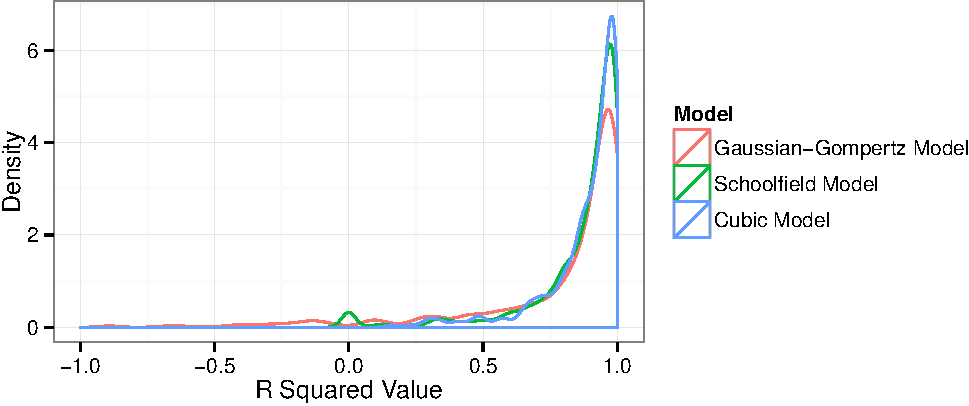
\includegraphics[scale = 1]{r_distr.pdf}
\caption{Spread of the \(R^2\) values for the different models.}
\label{fig:r_distr}
\end{center}
\end{figure}

By defining a "good" fit to be one with greater than 0.75 \(R^2\) value, we can then determine the total number of models in every dataset that produce good fits (Figure \ref{fig:bar}). Unsuprisingly given the \(R^2\) distribution, the number of poor fits in the Gaussian-Gompertz model was far higher than for the other two, with the cubic model appearing slightly more successful than the Schoolfield model for producing good quality fits. Again, this can be attributed to the higher-power terms in the cubic function. Using the AIC and BIC as measures of the quality of a the model allows us to select the best model for each dataset (Figure \ref{fig:pie}). 32\% of datasets had the best fit with the Schoolfield model, 22\% with the Gausian-Gompertz model and the remaining 46\% saw the best fit with the cubic model.

\begin{figure}[h]
\begin{center}
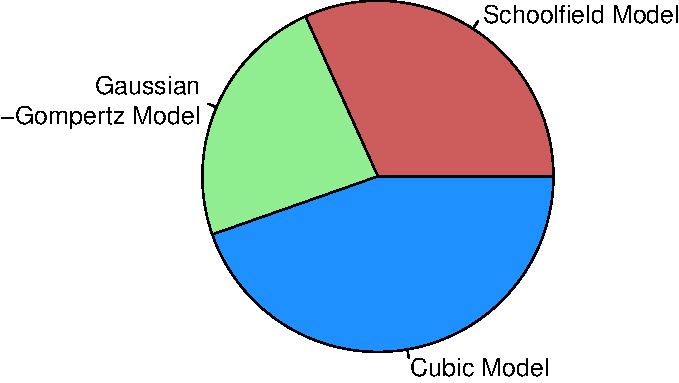
\includegraphics[scale = 1]{pie.pdf}
\caption{Best model selection for the datasets.}
\label{fig:pie}
\end{center}
\end{figure}

\begin{figure}[h]
\begin{center}
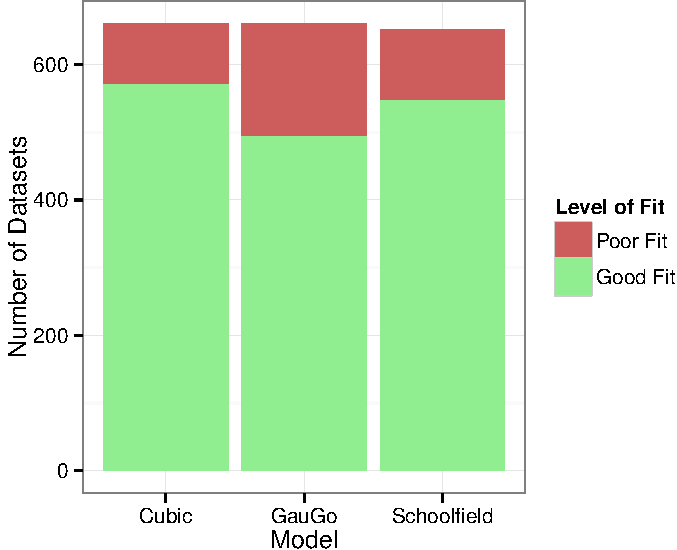
\includegraphics[scale = 1]{bar.pdf}
\caption{Number of datasets that produce good and poor fits for each model category.}
\label{fig:bar}
\end{center}
\end{figure}

\begin{figure}[h]
\begin{center}
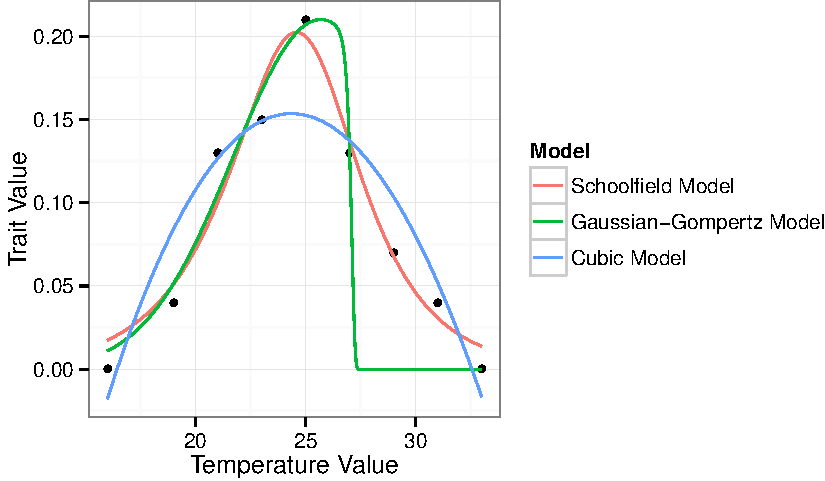
\includegraphics[scale = 1]{poor_cubic.pdf}
\caption{Examples of varying strategies of fits for different models. }
\label{fig:poor_cubic}
\end{center}
\end{figure}
\begin{figure}[h]
\begin{center}
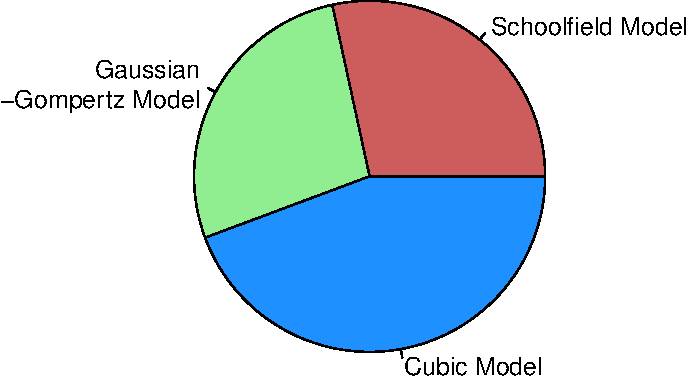
\includegraphics[scale = 1]{high.pdf}
\caption{Best model selection for the datasets with more than 15 data points.}
\label{fig:high}
\end{center}
\end{figure}
\begin{figure}[h]
\begin{center}
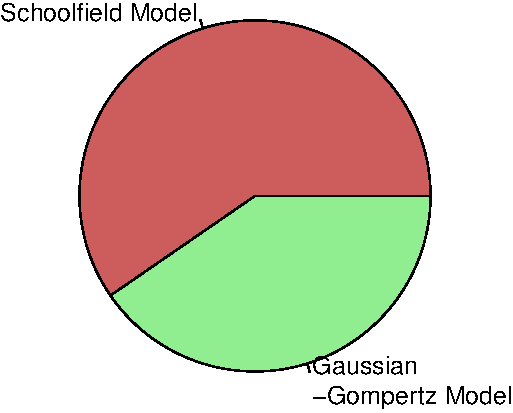
\includegraphics[scale = 1]{remove_cubic.pdf}
\caption{Best model selection between Gaussian-Gompertz and Schoolfield models.}
\label{fig:remove_cubic}
\end{center}
\end{figure}
\FloatBarrier
\section{Discussion}
From much of the data produced, it appears that with a better distribution of \(R^2\) values, the cubic model produces the best fit for the most datasets. However, as the cubic model is entirely mathematical, with none of the terms having a basis in biological attributes, it makes producing a model for a different organism without full data very difficult.Contrastingly, given measurements of \(E\), \(E_D\), \(B_0\) and \(T_pk\), a Schoolfield model could be generated for any organism, outlining the advantage of a mechanistic model. 

Furthermore, many of the curves for cubic models, whilst producing a higher \(R^2\) value than the other models, had peaks far lower than the recorded maximal trait value and produced a curve which likely wouldn't work if there were more data points recorded. It could be argued that for many datasets, including those for \textit{Pandorina morum} (Figure \ref{fig:jumps}) and for \textit{Ostreopsis siamensis} (Figure \ref{fig:poor_cubic}), the cubic fit does not produce biologically accurate curves. The smooth curve does not peak near the value for the recorded maximum trait, and the curve falls off extremely quickly at the minimal trait values. For temperatures outside the range of those recorded, this would mean high negative trait values, which would be very unlikely biologically. The tapering curves displayed at extreme temperature values by both the Gaussian-Gompertz and Schoolfield models would be far more likely to accurately fit experimental data.

Nevertheless, in terms of raw fitting ability over the datasets provided, the \(R^2\) distribution and AIC values of the models leads to our conclusion being that the non-mechanistic cubic model best fits the data. Interestingly, when the best model is calculated just for models with more than 15 datasets, the proportion of datasets best fitting each model does not change much (Figure \ref{fig:high}). This is potentially due to clustering of the data points in the optimum range, meaning that extreme values of temperatures aren't as important when calculating the best fit, removing the advantage that might have been predicted for the Gaussian-Gompertz and Schoolfield models.



Even so,the advantage of having a mechanistic model can be hotly debated \citep{OConnor2007},  especially as the data provided here has the Schoolfield model generally producing a better fit than the counterpart phenomenological model, the Gaussian-Gompertz model. If we remove the cubic model as a comparative, a larger proportion fit the Schoolfield model (Figure \ref{fig:remove_cubic}). The spread of fits is also better, with Figure \ref{fig:r_distr} showing a greater peak for high \(R^2\) values for the Schoolfield model than the Gaussian-Gompertz model. 

Overall the results suggest that mechanistic models have great potential to accurately fit thermal responses in phytoplankton as well as providing a biologically meaningful basis for the model. Similar model fitting for experiments with a greater number of data points over a larger range of temperature values would provide insights into the predictive level of the models produced already. These models could help indicate whether the cubic model is actually as powerful a tool as highlighted here, and possibly give further reasoning behind choosing mechanistic models for thermal responses.



\FloatBarrier
\bibliographystyle{plainnat}
\bibliography{../References/CMEE-TemperatureResponse.bib}
\end{document}
